\documentclass{../sty/acm_proc_article-sp}
\usepackage[T1]{fontenc}
\usepackage[bitstream-charter]{mathdesign}
\begin{document}


\title{Unwrangled Data to Normalized SQL}
\subtitle{Project Proposal}

\numberofauthors{1} 
\author{
\alignauthor
Eden Zik and Kahlil Oppenheimer\\
       \affaddr{Brandeis University}\\
       \affaddr{415 South St. Waltham MA}\\
       \email{\{edenzik, kahlil\}@brandies.edu}
}

\date{\today}


\maketitle

\begin{abstract}

Data analysis tools are extremely high in demand. However, one known issue with data analysis is an inconsistency in formatting between different data sources. Is my data compatible with the analysis tool I'm trying to use? This problem is only exacerbated when data is represented inconsistently between various mediums. Take for example a team of two, each trying to represent the same structured data. Let's say that one person decided to create an Excel spreadsheet while the other wrote a Python script to populate a CSV file. What if they chose inconsistent names of attributes for enumerated types (i.e. ``female'' vs. ``f'' vs. ``Female'')? What if one person decided to leave some cells blank, while the other didn't? What if the person entering into Excel had typos that were corrupting various aggregation results? Suddenly, the team's simple task of trying to merge and aggregate their data with some analysis tool becomes much more complicated.

To deal with this, many analysts spend a significant amount writing various scripts to transform multiple data sources into one standard. This ``data wrangling'' often requires manual transformations of columns and rows, correcting individual values, and aggregating data from multiple sources with different layout. Fortunately, two applications were created to aid this process along: Stanford's Data Wrangler and Google's Open Refine. Although both projects have been developed with a similar goal of a visual and intuitive interface for data wrangling, they create a short-term but not scalable solution. Both Data Wrangler and Open Refine export their ``wrangled'' result as one massive CSV file. This is fine for small-scale individual tasks, but this does not scale in the way that the modern world demands that data scale. Our project will take this output CSV and transform it into a specifiably normalized SQL relational database. This transformation will allow the user all of the well-known benefits of a relational database management system, such as referential integrity, data consistency, and easier compatibility with analysis tools. Our project aims to provide data analysts with the ultimate tool for normalization of structured but unwrangled data.

\end{abstract}




\section{Who are we?}

We (the authors of this proposal) are both undergraduate students studying Computer Science at Brandeis University. We've worked together extensively on many projects and have a great familiarity with one another's work habits. Because of this, there was no question in my mind that Eden's strengths would compliment my own in a way that would make this project possible.

Eden Zik is a double major in Computer Science and Biology. Eden has extensive experience with the open-source DBMS, PostgreSQL, and has written everything from queries and triggers to custom functions. Eden has also worked with many research groups (such as the Klausen Group) who struggle to effectively manage their data, which formed much of the inspiration for this project.

Kahlil Oppenheimer is a double major in Computer Science and Math. Kahlil has done work on the query optimizer team at HP Vertica, the company responsible for a commercial implementation of a Column Store (C-Store) analytics DBMS. Kahlil also wields a constructive skepticism that continues to whittle this project into its final (and hopefully best) stages.


\section{Current Problem}
Manipulating data is difficult. Developers and analysts often spend far too much time trying to write custom programs and scripts to fit their data into specialized analysis tools. Even when they successfully write these scripts, as the nature of the incoming data changes, the scripts must be modified in an unstructured, unscalable fashion. ``The result is that people with highly specialized skills (e.g., statistics, molecular biology, etc.) spend more time in tedious `wrangling' tasks than they do in exercising their specialty'' \cite{2011-wrangler}.

In addition, it is often the case that sources in formats appropriate for small-scale data analysis such as Excel, XML, or CSV outgrow their respective mediums and the need for a relational database becomes paramount. However, this transition from small-scale data to a relational database is non-trivial, which underscores the problem that our project is trying to solve.

\section{Existing Solutions}
Luckily, the aforementioned problem has been addressed and even partially solved. We will now describe the existing solutions, then we will follow by describing what they do not accomplish, i.e. what we will accomplish with this project.

Open Refine (formerly a Google project called Google Refine) is a data cleanup and reorganization tool developed for the purpose of cleaning up messy and inconsistent data from a CSV/Excel source. Open Refine uses its several subcomponents to process inconsistent spreadsheet data given user-defined heuristics such as regular expressions, filters, and manual cell-by-cell edits \cite{Refine}. The result is a spreadsheet which can then be visualized or further analyzed using Excel or R, respectively.

Data Wrangler is a similar tool implemented by The Stanford Visualization Group. Data Wrangler is based on a research paper published by the Stanford Visualization Group (now the University of Washington Interactive Data Lab) [INSERT PAPER CITATION]. Data Wrangler's website boasts that ``Wrangler allows interactive transformation of messy, real-world data into the data tables analysis tools expect'' \cite{wrangler-web}. Data Wrangler actually shares some functionality with Google Refine, such as the ability to analyze statistical frequencies to rework different names of the same semantic meanings into the same names (i.e. ``female'', ``Female'', and ``f'' all referring to the same semantic female).

The program helps users ``reformat data values or layout, correct erroneous or missing values, and integrate multiple data sources'' with an intuitive and visual interface. \cite{2011-wrangler}. For instance, users may have structured data with typos, missing fields, or just poor formatting. Data Wrangler suggests ways for the user to easily and intuitively correct these errors and ``wrangle'' their data into a structured and usable form. Data Wrangler also records the history of data transformations and allows users to preserve, analyze, and edit that history. The end result is that a user can take some structured, but not yet wrangled data, and manipulate it in an intuitive and reusable way, to one structured and wrangled data in a spreadsheet format.
The DataWrengler project itself is based on Potter's Wheel, an interactive data cleaning system described in a 2001 paper by Raman and Hellerstein \cite{raman2001potter}.

\section{Our Project}
Our project will take the spreadsheet format, normalize it into logical tables, and provide the ANSI SQL compliant set of transactions to populate a SQL database (SQL dump) with that data. Our project will use Data Wrangler to allow the user to ``wrangle'' their data into this one structured table of information, create a specifiably normalized schema based on that table to balance reduction of redundancy with query efficiency, and finally output the ANSI SQL compliant equivalent. In other words, users can go from structured but unwrangled data to a running SQL database with minimum difficulty.

\section{project relevance to databases}
We get to focus strictly on the logic of normalizing and generating database schemata, while still providing an application with practical use.
We get to focus strictly on the abstract logic because much of the low-level ``grunt work'' is done for us by Data Wrangler. In Data Wrangler's own words, we can spend our time ``exercising our specialty'', though through extending Data Wrangler rather than through using it.


Additionally, using an existing framework as base allows each stage of our project to be a functional application. The end result of our project will encompass a functionality that would have otherwise been impossible without the use of the Data Wrangler framework. With Data Wrangler covering the user interface and actual data wrangling, we can focus on powerful algorithms for normalization, while still providing an application that provides all of the aforementioned services. The end result is a final project that is interesting, usable, and directly relevant to database research.

\section{Technical Implementation}
While there are many ways to go about implementing our solution, we think we have come up with one that is both scalable and achievable within our time frame.

We will begin by forking the source code for Data Wrangler. Data Wrangler's licensing allows us to use and modify their code, so long as we meet minimal criteria (such as not associating our project with the name Stanford University).

We will initially preserve Data Wrangler's setup of being run entirely as front-end JavaScript code. While this has the disadvantage of not utilizing the full force of a back end, it has the advantage of a much lesser startup time, and lets us focus more on the actual database normalization component of the project. One future upgrade we'd like to implement, if time allows, is to move much of the service of the application to the server-side via NodeJS, a back-end JavaScript framework.

Using JavaScript for the entire application has the advantage of being extremely portable. JavaScript can be run in a browser (of course), but with recent technology from GitHub's Atom text editor, JavaScript can also be run on the desktop in a Windows, Mac OS, or Linux environment. This allows for portability unparalleled by most other programming languages.

Our project will also be extremely portable in regards to databases. For that reason, we're going to have our final result (a list of SQL transactions as a dump file) be compliant with the American National Standards Institute's (ANSI) SQL standard. This will allow for easier compatibility with any given DBMS (PostgreSQL, Oracle, SQL Server, etc.) with only minor translation for implementations that break the standard--but such translations probably already exist anyways.

With the project written entirely in Javascript and on top of Data Wrangler, we will be able to work at a high level of abstraction, maintain extreme portability, and work within an acceptable timeframe.


\section{Timeline}

\begin{description}
\item[Week 1 (10/06 - 10/12)]:
	\begin{itemize}
		\item Study the core code of Data Wrangler to gain understanding and familiarity
		\item Create our own instance of Data Wrangler running without modification in the browser on a server
	\end{itemize}
\item[Week 2 (10/13 - 10/19)]:
	\begin{itemize}
		\item Integrate features from Google Refine into project
		\item Support SQL output of denormalized data (assuming good structure, i.e. all columns have values)
		\item Have working alpha without normalization features
	\end{itemize}
\item[Week 3 (10/20 - 10/26)]:
	\begin{itemize}
		\item Design normalization algorithms
		\item Begin to Implement normalization as a feature
	\end{itemize}
\item[Week 4 (10/27 - 11/2)]:
	\begin{itemize}
		\item Finish implementing normalization algorithms
		\item Start writing tests for normalization features
	\end{itemize}
\item[Week 5 (11/3 - 11/9)]:
	\begin{itemize}
		\item Continue to test normalization features extensively
		\item Pass all test cases of normalization feature
	\end{itemize}
\item[Week 6 (11/10 - 11/16)]:
	\begin{itemize}
		\item Complete working beta with normalization features for public use
	\end{itemize}
\item[Week 7 (11/17 - 11/23)]:
	\begin{itemize}
		\item Release beta to test users and aggregate feedback
		\item Use feedback to make changes
	\end{itemize}
\item[Week 8 (11/24 - 11/30)]:
	\begin{itemize}	
		\item Use feedback to make changes
	\end{itemize}
\item[Week 9 (12/01 - 12/07)]:
	\begin{itemize}
		\item Code Lock
		\item Production Mode
		\item Documentation
	\end{itemize}
\item[Future work if time allows]:
	\begin{itemize}
		\item Redesign Graphical User Interface
		\item Move DataWrangler to backend via NodeJS
	\end{itemize}
\end{description}

\section*{Appendix A: Examples}
It is often the case that data collections outgrow their chosen medium, be it Excel, XML, or CSV. This growth is usually due to lackluster initial planning or limited familiarity with database technology.

A misfit of the data at hand and the method of aggregation (Excel vs SQL) can lead to a myriad of challenges. Said challenges can be made complicated if the database exceeds the limit for which manual data transformation are feasible.

We chose two brief examples to showcase the potential implications of early design decisions, their cascading effect on the database, and how we can solve them.

\begin{description}

\item[Referential Constraints] Spreadsheet formats are denormalized by nature, and the lack of foreign key constraints limits the ability of a table to minimize redundancy.

Given an excel spreadsheet consisting of one table. This table stores the names and addresses of all people who are customers of a bank and is taken from a known schema \cite{Mitch}:

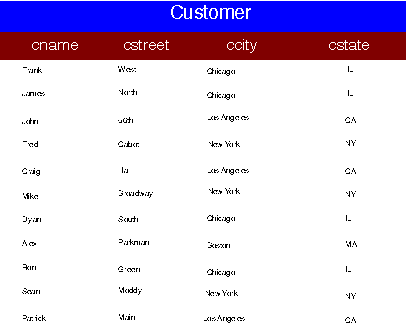
\includegraphics{../img/initial_table}

A design decision had been made to now use this customer table to store the account numbers of all customers. This decision had led the table to have an extra column containing an account number as well as a customers name and address:

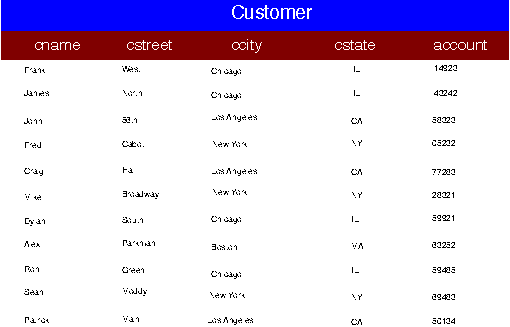
\includegraphics[scale=.9]{../img/second_table} 

The above table remains effective and fits within the limits of its medium (Excel). However, as an unforseen consequence of expansion, the bank began to offer multiple accounts to an individual. Some chose to get an account, while others did not:

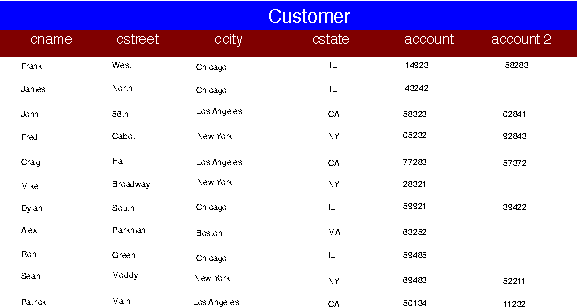
\includegraphics[scale=.8]{../img/third_table}

Although unappealing, the bank chose to add an entire column to the customer table in order to accommodate those with two bank accounts.

Inefficient, but necessary given the initial design decision. Shortly following:

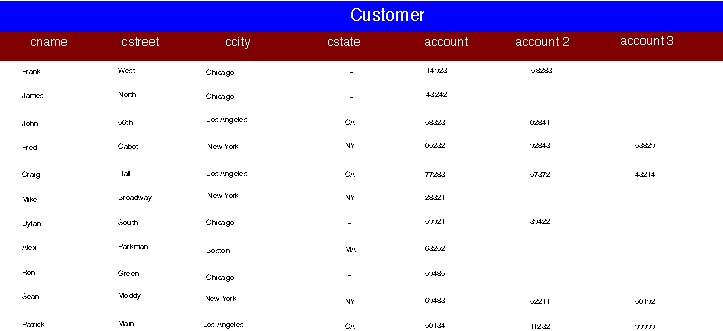
\includegraphics[scale=.6]{../img/fourth_table}

And quickly thereafter:

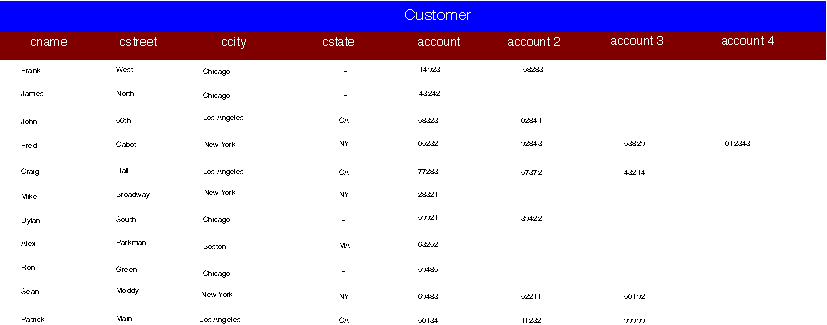
\includegraphics[scale=.53]{../img/fifth_table}

A single customer with 4 bank accounts had forced the bank to create an entire column.

Referential integrity is a textbook solution to this problem: offer a single table of customers with a foreign key to a table of accounts with an arbitrary number of accounts per person. However, given the large amount of data the bank has a difficult time transitioning to another medium.

Automation of the above above would enable the table to be normalized without a manual transfer of critical data (i.e copying the customers with multiple accounts to an auxiliary table one by one) which is prone to error.

The above example is a critical showcase our application's potential, and currently has no easy solutions.

\item[Inconsistency]

Data validation in spreadsheets is a well known and accepted feature, enabling a user to restrict the values of a cell to be within a predefined set. However, data validation encodings have the disadvantage of being completely unportable across platform (Excel $\rightarrow$ OpenOffice) or unsupported (CSV/XML).

We will now refer again to our bank example \cite{Mitch}:

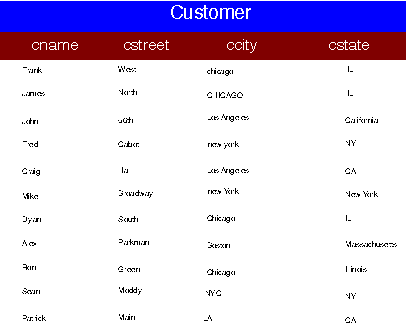
\includegraphics[scale=1.1]{../img/name_table}

While the semantics of a city and state in which a customer reside is identical, the strings in the table are not. This is a classic database problem which can be solved by either enumerated types or foreign key constraints.

The solution to this were described in both Data Wrangler and Open Refine: they enable you to consolidate all similar data types manually by frequency. The following is an example of this in Open Refine:

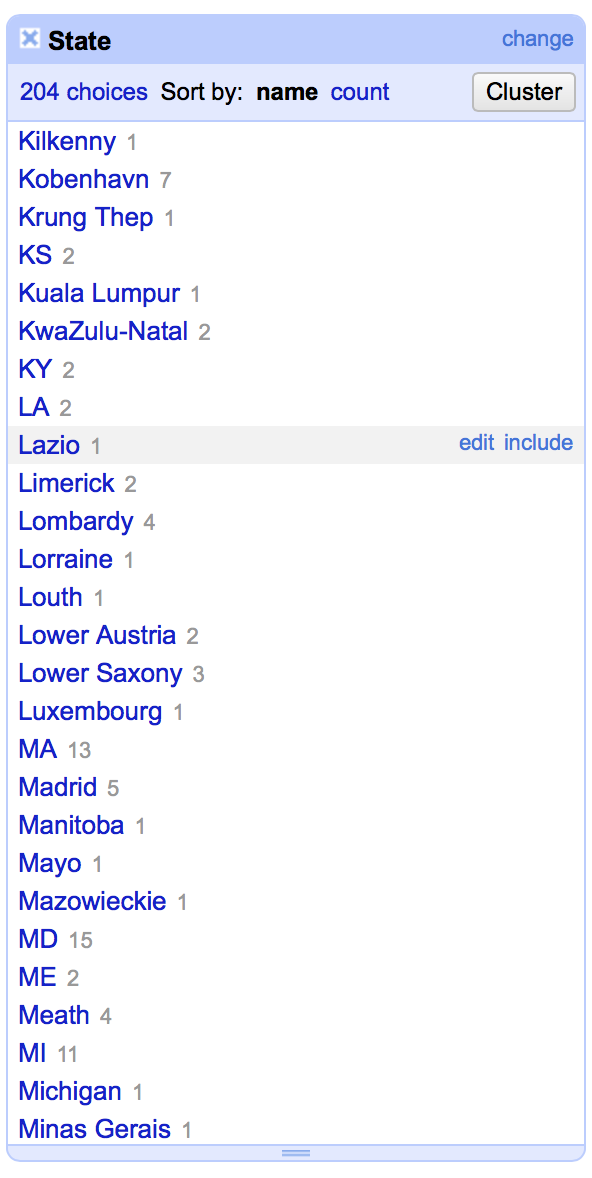
\includegraphics[scale=.5]{../img/refine}

Said implementation solve the problem at the current state of the database, but do not prevent future errors. Our SQL extension of the aforementioned solution will be an ultimate enhancement which will both consolidate the values onto the same semantics, but will also define a referential constraint/enumerated type in the schema definition it produces.



\end{description}

\section*{Appendix B: Interface}

As stated, we will root our entire codebase (interface included) on Data Wrangler. The user interface of Wrangler is as follows:

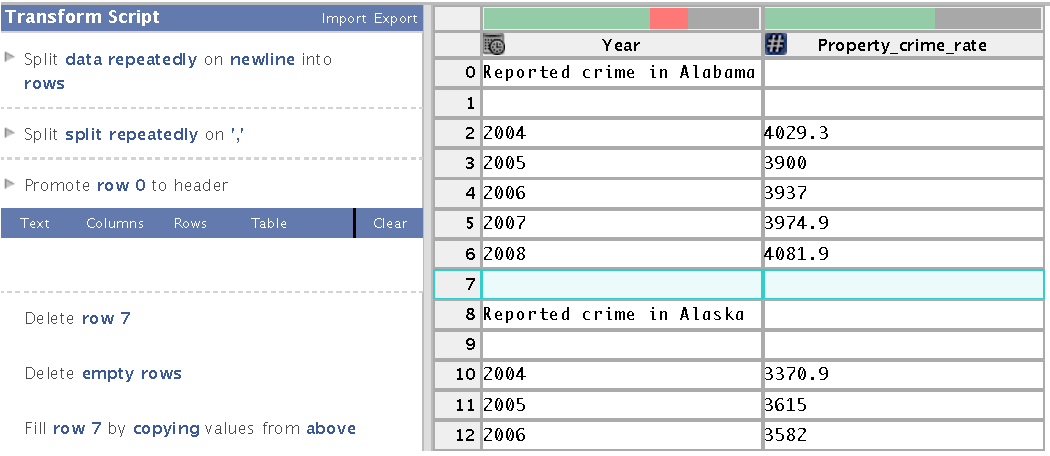
\includegraphics[scale=.44]{../img/wrangler_gui}

This interface is based on JavaScript panels. The left panel contains a history of all transforms done thus far, a selection menu, and automatically suggested transforms. We will integrate our SQL export function and normalization features within this paradigm, for it is established and shown to be concise, usable, and complete.


\newpage

\bibliographystyle{abbrv}
\bibliography{proposal}

%\balancecolumns 

\end{document}
